\section{Forensic case study: the \texttt{opus\_alias} arm}

\textbf{Setup.} The study's third tier was requested as a specific dated top-tier model, but the agent runtime accepts only an alias --- no dated identifiers --- so the request was unsatisfiable, and \emph{undetectably} so: nothing in the runtime's response surface reports which weights served a call. We label the arm \texttt{opus\_alias} throughout. Thirty invocations, ten each at three held-out cells ($N = 13, 21, 31$), predictions registered in \texttt{arm\_o\_preregistration.txt} before any sampling, digest \texttt{211718c6\bk b58d627f\bk 17e34aa7\bk 3ad6142b\bk 89c7f390\bk 48e5e19a\bk 8cc864d6\bk 3c281738}.

\textbf{Serving signature.} Completions returned in \textbf{2.8--9 s} across all thirty invocations. On the same harness and task the Haiku tier returned in \textbf{75--250 s} and Sonnet in \textbf{150--1170 s} --- one to two orders of magnitude slower for nominally smaller models, holding uniformly across all thirty invocations. This is a working-log observation (\texttt{STATE.md} \S8, \S8b), \textbf{not} captured in the released artifact: \texttt{arm\_f\_raw.json} rows carry exactly four keys (\texttt{arm}, \texttt{n}, \texttt{raw}, \texttt{sample\_id}), no duration field, and \texttt{arm\_f\_repro.py} contains no timing capture at all. A reader can recompute every validity figure and cannot check a single latency figure --- the one item of \S6's disclosure standard this paper does not itself implement (\S4.1's arms close the gap prospectively, not for these thirty rows). A second apparent anomaly (uniform reported-token counts, $\sim$49.9k across all thirty) is withdrawn: the harness logs a single aggregate usage figure over a large fixed system prompt and a task prompt uniform in length (520 characters) across cells, so near-uniformity is exactly what the design predicts, and the residual spread is plausibly tokenizer-level variation between ``13'', ``21'' and ``31''. No contemporaneous control exists: the three tiers were not interleaved, and load demonstrably varied within the study (five invocations elsewhere were rejected by a concurrency cap before reaching a model, \S6 item 3), so load cannot be excluded as a latency contributor. Speed is not precision on the one stack we fully control --- across \S3's ladders throughput does not order by bit-width (14B Q8\_0 slowest of four rungs at 14.9 tok/s against Q2\_K's 22.5; 7B FP16 slower than every quantized rung; \S6 \texttt{sec6\_cv\_canary\_audit.py}). Those gaps are tens of percent against this arm's one-to-two orders, so the magnitudes are not comparable. But speed and precision are demonstrably separate axes even on a fixed stack, and throughput is not a portable fingerprint --- it is not stable across hardware either (\S6 item 4).

\textbf{Behavioral signature --- recomputable, both tolerances.} Validity was \textbf{4/30 (13\%)} at 1e-6 and \textbf{4/30} at strict 1e-9 (per cell 3/10, 1/10, 0/10) --- tolerance-invariant collapse. Comparators, recomputed from the released file: Sonnet \textbf{30/30 at 1e-6, 27/30 at 1e-9}; Haiku (\texttt{bare}) \textbf{50/60 at 1e-6, 47/60 at 1e-9}. A fourth comparator, present in the released file and not previously reported: 70 \texttt{trace} rows at the same three cells (20, 30, 20), belonging to the companion paper's trace-elicitation arm, score \textbf{63/70 valid (90\%)}, per cell 18/20, 28/30, 17/20 --- against \texttt{opus\_alias}'s 4/30, Fisher $p = 1.1\times10^{-13}$; pooling all three comparators, 143/160 against 4/30, $p = 1.0\times10^{-16}$ (comparators do not differ detectably from each other: \texttt{trace} vs \texttt{bare} $p = 0.30$, vs Sonnet $p = 0.099$). Its prompt is substantially different from the bare prompt while the serving path is the same one the other local arms used, so a large prompt change produces nothing resembling the collapse --- a control \S4 otherwise lacks. Two caveats: this arm is a reuse from the companion paper's question, and \texttt{arm\_f\_raw.json} does not distinguish that paper's pilot rows from its \texttt{trace\_v2} rows, which it forbids pooling --- the 63/70 above therefore pools rows the companion paper forbids pooling, because the released file provides no separating field. No claim in \S4 rests on it; the 4/30 against 30/30 and 50/60 contrast stands without it. (A 45-row prior Haiku slice that once served as comparator was overwritten in place by a later 100-invocation wave with colliding \texttt{sample\_id}s and no batch/date field, and cannot be reconstructed --- the concrete case motivating \S6 item 3.)

The failures are geometric, not formatting: all 26 invalid rows overlap (2 additionally contain zero-radius circles, but both still overlap once those are removed --- gate ordering, not disjoint failure modes; one, $N = 21$ sample 5, has 12 of 21 radii at zero). The errors sit far outside rounding noise (one $N = 31$ row: a deficit of 0.06 against tolerance 1e-6, $\sim$6$\times10^{4}$ times over). The attempted constructions shifted family and are \emph{more} ambitious than the grid-plus-filler templates the other tiers produce: at $N = 13$, all ten rows place four $r = 0.25$ corner circles plus filler radii in an Apollonius-like arrangement (classifier returns \texttt{structure: other} for all ten); at $N = 21$, mixed-radius grids with fillers; at $N = 31$, a coarse $r \approx 1/6$ grid with border strips. The four valid samples score below the registered trap value by very different margins --- at $N = 13$, 1.2646/1.2873/1.4142 against a 1.625 trap (13--22\% below); at $N = 21$, 2.07 against 2.1 (1.4\% below, effectively at it). Registered scorecard: P-O1 (on-trap rate $\le$ Sonnet's 1/30) \textbf{held} at \textbf{0/30} --- nearest miss 2.07 against 2.1, off by 0.03, fifteen times the registered 2e-3 window; P-O3 (multi-radii fraction $\ge$0.9) \textbf{held}, 4/4; P-O2 (rival-argmax) and P-O4 (best valid score $\ge$2.2588835) \textbf{failed} outright (0 rival-argmax against Sonnet's 6/30; best 2.07 against the required value) --- two held, two failed, none unevaluable.

\textbf{Two hypotheses.} H1, \emph{serving-path degradation}: a fast decode path erodes the arithmetic precision needed to close a tangency while leaving construction choice intact --- precisely \S3's signature. H2, \emph{genuine tier property}: the resolved weights really do attempt harder constructions and execute them less reliably. \textbf{What the observable set can and cannot separate.} The runtime exposes, per invocation, exactly four things: completion text, wall-clock duration, an aggregate usage figure, error codes (call this set \emph{O}). On text, both hypotheses induce the same distribution. On timing they are not symmetric: H1 predicts the latency observation directly; H2 needs an auxiliary --- ``a fast path was in use but had no behavioral effect'' --- which is H1's mechanism minus its causal claim, strictly more complex. The observations mildly favour H1 within this snapshot, but cannot \emph{decide}, because the auxiliary is not itself testable through \emph{O}: no element reports which decode path served a call. \textbf{The irreducible residue is the unattestability of the serving path, not a blanket impossibility of behavioral discrimination.}

A pinned dated endpoint, outside the agent runtime, would be informative in both directions but cannot attest what the \emph{alias} resolved to on the day sampled --- the counterfactual is gone. We did not run this experiment; its absence is a limitation of this paper. Two further routes were named but not run in earlier drafts and have now been run (\S4.1): \textbf{prompt variation} (hand the alias a fixed, known-valid packing and ask it to verify/repair --- decoupling execution from ambition), and \textbf{a dated re-snapshot} (re-sampling the same alias later, informative either way, without ever attesting either snapshot's serving path).

\subsection{Both follow-ups, run}

Preregistered together in \texttt{arm\_r\_preregistration.md}, committed before the first invocation, run on 2026-08-07 through the same alias. Ninety invocations: thirty re-issuing the byte-identical bare prompts (\textbf{arm B2}), sixty on the repair task (\textbf{arm R}), split across two cells, a three-step precision ladder, and two tiers. All figures replay from \texttt{arm\_r\_analysis.py}.

A repair score without an anchor would be uninterpretable --- arm B2 is the anchor, registered as P-R0 at \textbf{$\le$ 12/30 valid}, disconfirming branch written out in advance.

\textbf{Arm B2 disconfirmed P-R0 at the widest margin the design allows:} $N = 13$, 3/10 $\to$ \textbf{10/10} (best valid 1.776141); $N = 21$, 1/10 $\to$ \textbf{10/10} (2.276800); $N = 31$, 0/10 $\to$ \textbf{10/10} (2.794180); pooled 4/30 $\to$ \textbf{30/30}, Fisher $p = \mathbf{7.8\times10^{-13}}$. The $p$-value rejects the hypothesis these are draws from one success rate; it is \textbf{not} a test that the serving path changed (one path per condition --- pseudoreplication with respect to that question).

Wall clock and usage were logged as two further channels, and they diverge. Wall clock went from 2.8--9 s to \textbf{68.7--594.1 s} (median 228.2), overlapping the comparator range it was once one to two orders below, but this comparison is uncalibrated in both directions (eyeballed log ranges vs a runtime-reported field, no contemporaneous 2026-08-07 comparator, no timing claim registered) and is consistent with, not evidence for, the validity change. The usage channel fails entirely, and instructively: reported usage went from uniform $\sim$49.9k to 58k--195k, a 3.35-fold spread that looks like a second signature, until arm R's same-day, same-alias, different-task rows show usage uniform to \textbf{1.01-fold (54{,}377--54{,}803)}. The spread tracks the task, not the date (within B2, usage and duration correlate at $r = +0.69$). \textbf{The usage observation is withdrawn again, here.}

\textbf{What the surviving result does not do:} retract any 2026-08-01 observation. \textbf{What it does:} take the section's question away rather than answer it. H1 and H2 remain well-formed about the 2026-08-01 call; what is gone is any route to testing them, because the only handle --- the alias --- no longer addresses that call, and no observable reports when it changed. A later call is a sample of an unknown condition, not a second sample of the same one. Fast-and-13\% then slow-and-100\% is what H1 predicts if only the decode path moved, and equally what H2 predicts if the weights themselves changed; two conditions, no randomization, and a simultaneous difference in date, load, decode path and possibly identity distinguish none of these.

\textbf{Arm R ran anyway, because it was registered.} Six cells --- $N \in \{13, 31\} \times \delta \in \{$1e-2, 1e-3, 1e-4$\}$ --- five invocations each at alias and Sonnet, on a grid-plus-interstitial packing exactly tangent everywhere with one circle slid by $\delta$. Results: \textbf{59/60 exact} (all 5/5 except alias $N=31$, $\delta=$1e-3 at \textbf{4/5}), recall 1.00 in every cell of every tier, the single miss a near-miss false positive (true clearance 7.089e-04), zero empty responses anywhere, detection flat in $\delta$ across two orders of magnitude at both tiers. Of seven registered predictions, three held, four failed: P-R1 (exact $\ge$0.6 at $\delta=$1e-2) held; P-R5 (Sonnet $\ge$ alias at $\delta=$1e-2) held; \textbf{P-R4 held vacuously} (predicted empty responses would not become rarer --- there were zero anywhere); P-R2 (``monotone non-increasing,'' satisfied by flat detection) scored FAILED on one cell only ($N=31$'s 1.0/0.8/1.0, the single false positive making the sequence rise); P-R3 ($\ge$2/5 drop $\delta=$1e-2$\to$1e-4) and P-R6 (Sonnet beats alias at $\delta=$1e-4) both failed outright --- P-R6 became structurally unreachable once Sonnet hit ceiling.

\textbf{The H1 signature the probe was built to detect was not detected --- weaker than absent, and it matters at this size.} Five invocations per cell put the one-sided 95\% lower bound of a 5/5 cell at 0.549; the design excludes a precision effect of roughly 45 points or more and says nothing about a smaller one. \textbf{And we may not read it}: P-R0's failure triggers the registration's fourth branch --- arm R measures a serving path that cannot be tied to the 2026-08-01 one, so no H1/H2 conclusion is drawn from it, even though arm R's own result is clean and would otherwise read as evidence against H1. Two things arm R does establish on the path it actually measured: repair-style probes are not where this path fails on this substrate ($\delta=$1e-4 at $N=31$, four orders below coordinate scale, found by 5/5 both tiers), and there is no tier contrast left to measure here, since both tiers sit at ceiling. Registered predictions P-O2/P-O4, refuted on 2026-08-01, are not rehabilitated by 2026-08-07's numbers --- they were registered about a path no longer addressable. Arms B2 and R capture per-row duration and usage, closing \S6's disclosure gap prospectively (not for the original thirty rows).

\section{What is repairable and what is not}

The repairs below are implemented in \texttt{arm\_f\_repro.py} and companions, not merely proposed, and where they are not, this section says so.

\textbf{Implemented.} Prompt text is pinned and SHA-256 hashed before any sampling, one hash per problem size: $N = 13$ \texttt{32db485b\bk ea625ff9\bk f39f4723\bk ebf1a01f\bk 337559a9\bk e2cf567f\bk b486928f\bk 71f7f8df}, $N = 21$ \texttt{a415425b\bk 4ed5a57e\bk a9b6f09c\bk 2328508f\bk 12370e16\bk 24734e1c\bk 5ed32913\bk 741795a9}, $N = 31$ \texttt{a664d003\bk cbf1c0ec\bk a51bae5b\bk 3a1d0720\bk 71eb3475\bk 6725a749\bk 1d6a2e8f\bk a3b78e92}. (Each prompt is 520 characters, template plus two-digit $N$. \texttt{arm\_f\_prompts.json} carries five cells --- $N = 13, 17, 31, 35, 37$ --- verifying the $N = 13$ and $N = 31$ digests directly; $N = 21$ is absent from that file but checkable, since substituting ``21'' for ``13'' in the released $N = 13$ prompt reproduces \texttt{a415425b...} byte-exactly.) Every raw output is stored verbatim, parsed or not. Scoring, validity and construction classification are deterministic, local, computed at both tolerances per row. Predictions with explicit falsifiers and a disconfirmation rule are written before the first invocation and externally timestamped; \S4 publishes the full registration digest.

\textbf{Implemented partially, and named.} Run date is recorded with the alias$\to$dated-id mapping in force that date, but the released map contains a single entry (for the Haiku proposer), and \texttt{RUN\_DATE} is a single hard-coded date that is \emph{not} the \texttt{opus\_alias} arm's actual run date. The paper's headline provenance repair is unimplemented for precisely the arm the paper is about. Raw storage has a matching defect: rows carry no batch, wave or run-date field, and \texttt{sample\_id} collides across arms and waves, so the released file cannot be sliced back into the arms as originally reported.

\textbf{Not repairable from inside.} Sampling parameters (temperature, top-p, top-k) are not exposed and are the parameters that shift the output distribution most. The alias$\to$weights binding is a promise, not a hash, repointable at any time; past runs cannot be re-executed against the weights that produced them. The subagent inherits a system prompt and user-level instruction files, not part of the task prompt and not held fixed across time. The serving path is not attested at all --- no flag distinguishes fast-mode from standard decode, the exact variable \S4 needed and could not obtain.

\textbf{Does output-text fingerprinting close the gap?} \citet{wimbauer2026fingerprintinginferencesystemslarge} show serving-stack differences are detectable from output text alone, but three things keep it from settling \S4 as run. Fingerprinting is \emph{classification against reference signatures}, and none exist for this vendor's closed serving paths. A tempting-but-wrong objection is that the arm's thirty completions (mean 578 characters) are too thin: these methods issue \emph{fresh} probes against a live alias, so the relevant budget is queries one is willing to spend, not stored text (\citealp{leshin2026behavioralfingerprintsllmendpoint}, fingerprint from fixed-prompt output distributions and detect changes of inference stack and quantization, and \citealp{bruckner2026tokenenoughfingerprintingverifying}, recovers model identity from roughly a hundred single-token queries; both are affordable). What survives is only retrospective: fresh probes cannot be sent to the path that answered our thirty calls in the past, because it is no longer addressable. Most fundamentally, a positive fingerprint would identify a \emph{stack}, not attest \emph{weights} --- it could strengthen H1's antecedent without touching the auxiliary H2 needs. Fingerprinting is the most promising published route to narrowing this class of question, is not runnable on this corpus, and a study banking reference signatures while the endpoint is available would be a genuine advance over what we did.

\begin{longtable}{@{}p{0.18\textwidth}p{0.1\textwidth}p{0.32\textwidth}p{0.32\textwidth}@{}}
\caption{Repair protocol: which observability gaps are repairable from inside the
runtime, by what mechanism, and what residual risk survives the repair.}\\
\toprule
Item & Repairable? & Mechanism & Residual risk \\
\midrule
\endfirsthead
\toprule
Item & Repairable? & Mechanism & Residual risk \\
\midrule
\endhead
Prompt text & Yes & SHA-256 pre-sampling, digests published & None \\
Raw outputs & Partial & Verbatim storage, failures included & No batch key; \texttt{sample\_id} collides across waves \\
Scoring / classification & Yes & Deterministic local evaluator, both tolerances & None \\
Predictions & Yes & Hash-locked prereg, externally timestamped & Registration errors --- disclose, don't amend \\
Model identity & Partial & Alias + run date + dated-id map in force & Map covers Haiku arm only; \texttt{RUN\_DATE} wrong for \texttt{opus\_alias}; alias may be repointed \\
Serving-signature stats & Partial & Absent from \S4's arm, implemented in \S4.1's & \S6 item 4's firing condition tested against \S3's own rows and withdrawn; disclosure half retained \\
Sampling parameters & No & --- & Unknown distribution shift \\
Alias $\to$ weights binding & No & --- & Silent substitution; past runs unrepeatable \\
Serving path (fast-mode) & No & --- & \S4-class confound; fingerprinting not runnable on this corpus \\
Inherited system/user prompt & No & --- & Unlogged context drift \\
\bottomrule
\end{longtable}

\textbf{The scorer is model-written, and that is a circularity worth naming.} This paper's integrity argument rests on deterministic local scoring, but that code was written with assistance from models in the same family as the runtime \S4 studies. The available answer is reimplementation: \texttt{sec3\_ladder\_repro.py} was written independently, from the definitions in the text, and re-derives \S3's 14B figures and five of nine Fisher tails; \texttt{sec3\_7b\_repro.py} replays the rest; \S4 was re-scored from \texttt{arm\_f\_raw.json} by a separately written geometric checker. Agreement is exact except the one invalid-row near-copy count noted in \S3.1. This is not independence in the strong sense --- the same author directed both implementations --- but it establishes that figures follow from the released rows under stated definitions rather than a particular scorer's quirks.

\section{Implications}

Every LLM-evolution, best-of-$N$ and iterative-refinement study run through a managed agent harness inherits this list --- FunSearch-style program-evolution loops, self-refinement pipelines, tier-ladder comparisons naming ``the model'' by alias. Such studies are not thereby wrong; they are unrepeatable in a specific, now-demonstrable way, and \S3 establishes that served weight precision is \textbf{one} unrepeatable variable the outcome is sensitive to. Whether others behave alike is a hypothesis raised, not tested. The correct response is disclosure, not retraction.

\textbf{The capability alternative, tested and bounded (wave 4, registered).} The strongest alternative reading of \S3 --- echo is what any weak proposer does, so a weak model rather than a 2-bit rung would suffice --- was left standing because no prior experiment varied capability independent of precision. Wave 4 did (\texttt{wave4\_prereg\_tiers\_heilbronn.md}, SHA-256 \texttt{7b3e67dc...}, published before sampling): three hosted capability tiers ran the identical Heilbronn $n=13$ lineage protocol, same seed parent, same echo definition, tools forbidden (\texttt{tool\_uses} 0/120). \textbf{Result: 0/120 coordinate-verified echoes --- every tier at 0\% against a registered $\le$30\% bound --- verdict DISSOCIATION} (roughly a 3\% bound at this $n$, not an exclusion at any rate). The registered secondary (echo monotonicity across tiers) returned \textbf{NOT EVALUATED} (its 10-echo floor unmet). No proposal in any tier improved on the seed (0/120; wave 3's GPU ladder later went 0/495 on the same task and parent --- substrate-independent stall). The sharper finding: \textbf{the tiers fail differently, not less.} Stuck GGUF rungs echo at 46.9--63.1\% (\S8), stuck hosted tiers at 0\% (though on LABS, a third task, stall-echo rates \emph{reversed}, \S8 --- Heilbronn-specific, not a law of stalls). The registered template check finds valid outputs scoring exactly zero (three-plus collinear points) at 52.5\% for the weakest tier, 27.5\% for the middle, and \textbf{97.5\% for the strongest}, whose 39/40 zero-scoring outputs are family-similar symmetric lattices, pairwise distinct at 6 dp. The 2-bit rung's signature failure is \emph{copying the parent shown}; the hosted tiers' signature failure is \emph{ignoring the parent and emitting a template}. A capability ladder does not reproduce the quantization ladder's failure mode even where it fails more often. Scope limits are the prereg's own: served precision, sampling parameters and serving path per tier are unattested (C3); one date; one harness wrapper; and the dissociation bounds the capability confound over the tiers sampled only.

\textbf{A minimum disclosure standard --- mostly an endorsement, with one addition.} GUIDE-LLM (Feuerriegel et al., \emph{Nature Human Behaviour} 10:1182--1186, 2026), a 14-item consensus checklist from an 80-expert panel, already mandates exact model version and access method, prompts and system instructions, sampling parameters, validation; parallel software-engineering guidance exists \citep{baltes2026guidelinesempiricalstudiessoftware,korn2026reportingllmpromptingautomated}, and \citet{siddiq2025largelanguagemodelssoftware} show artifact badges across 640 papers do not guarantee reproducibility. Items 1--3 below restate requirements those documents already impose, with agent-runtime specifics.

\textbf{Item 4 is the addition, and the artifact that motivated \S4 does not implement it} --- \S4's central evidence is a working-log observation rather than a checkable file, while \S4.1's arms implement it and the value of doing so is visible: the serving-signature change those arms document is checkable in a way \S4's is not.

\begin{enumerate}
\item \textbf{Alias, run date, and the alias $\to$ dated-id map in force on that date.} Two lines of the harness header; pins nothing but converts an unfalsifiable claim into a dated, checkable one. Implemented here for one proposer only --- a map omitting the arm under study is not provenance (\S5).
\item \textbf{Prompt hashes computed before sampling, and published in the paper} --- a digest kept in a private file is a check, not a disclosure (\S5 publishes ours).
\item \textbf{Verbatim raw outputs, including failures, with a batch key.} In our own logs, five invocations were rejected by a concurrency cap before reaching a model in the Haiku wave; scoring them as proposer failures would have moved that arm's reported validity from 32/45 (71.1\%) to 32/50 (64.0\%) --- 7.1 points absolute, 10.0\% relative (this worked example uses the superseded 45-row slice, no longer reconstructible after an in-place overwrite --- the overwrite is itself an instance of the defect this item exists to prevent). The batch key is the part we got wrong.
\item \textbf{Serving-signature statistics, with a firing condition.} Per-invocation duration and usage, logged and reported as distributions with an explicit canary condition: flag an arm when duration CV falls below one third of a neighbouring tier's on the same cells, or median duration differs by more than an order of magnitude under a same-window interleaved schedule; disaggregate usage before reporting spread.

\textbf{We then ran item 4 against our own data, and it has a false-positive mode.} \S3's ledgers carry per-invocation \texttt{wall\_s} on a \emph{fixed} inference stack (fixed llama.cpp build, single P100, same sampling parameters, same harness), so whatever the canary reports there is not a serving-path change (\texttt{sec6\_cv\_canary\_audit.py}). \textbf{It fires}: duration CV among valid rows is 0.0603 (Q4\_K\_M) vs \textbf{0.0143} (Q2\_K), ratio 0.237, below the one-third threshold; wave 2 replicates, 0.0692 vs \textbf{0.0200}, ratio 0.289 (permutation $p < 0.0001$ both waves); Q3\_K\_M does not fire on either wave (ratios 0.949, 1.066) --- the canary is selectively wrong at exactly the rung \S3 is about. \textbf{The mechanism is output degeneracy, not serving}: splitting rows by echo status, duration CV is low among echo rows at every rung (Q4\_K\_M 0.0210 on $n=34$, Q3\_K\_M 0.0141 on $n=31$, Q2\_K 0.0113 on $n=46$) and high among non-echo rows at every rung (0.0783 on $n=31$, 0.0778 on $n=20$, 0.0294 on $n=3$) --- an echo re-emits its parent verbatim, lands on the same token count, takes nearly the same time. Q2\_K's aggregate CV is low because 46 of 49 valid rows are echoes, a property of the output, not the serving path. \textbf{Item 4 needs a control it did not carry}: report duration dispersion conditioned on output identity, or exclude repeated outputs before computing CV. This does not overturn \S4, whose evidence is an absolute one-to-two-orders-of-magnitude latency gap on a non-echoing arm (4/30 valid), but it is a competing explanation \S4 never named for the class of evidence it relies on.

\textbf{The repair fails, in a way that matters more than the repair would have.} Removing the confound --- throughput over non-echo valid rows only --- looked disjoint on wave 2 (Q4\_K\_M [17.911, 18.126], Q3\_K\_M [15.731, 15.938], Q2\_K [16.596, 16.718] tok/s). Three things break it. First, \textbf{wave 1 is not disjoint}: its Q4\_K\_M range [16.455, 18.188] entirely contains Q2\_K's [16.703, 16.753], and an earlier draft quoted only medians, hiding the overlap. Second, \textbf{a cold-start effect silently did the filtering}: the first invocation against each parent runs at $\sim$92\% of steady-state throughput uniformly across all twelve rung$\times$wave cells (0.918--0.929), and on wave 2 every cold row happens to be an echo or invalid, so the echo filter removed them by accident, making ``non-echo'' silently a \textbf{warm} set --- a verifier's fresh probe is always cold, so it would read the 92\% band, not the published one. Third, \textbf{the band does not survive a hardware change, and the order inverts}: the same SHA-256-pinned Q2\_K file runs 16.62 tok/s on the P100 and 22.48 on 2$\times$T4 (Q4\_K\_M: 17.94 and 21.45); on the P100 Q4\_K\_M is faster, on the T4s Q2\_K is faster, not a shifted scale but an inversion. Throughput is also length-dependent (within-rung correlation between completion length and tok/s $\approx -0.9$), which fixes none of the three. These three mechanisms are the transferable part for anyone attempting timing-based attestation: dispersion is confounded by output identity, warm-up gradients can masquerade as between-condition effects and vanish by accident under an unrelated filter, and a per-file timing band inverts across hardware --- structural, and the case where the verifier does not control the hardware is exactly the attestation case. What this licenses about C3, stated narrowly: it does not show no observable attests the served file (output-side methods exist, \S7), only that \textbf{the one instrument class a verifier can compute from what an agent runtime already returns --- timing --- is ruled out}, worsening when the verifier loses the hardware. What survives: throughput does not order by bit-width on either ladder (14B: Q8\_0 slowest at 14.91 tok/s against Q2\_K's 22.48; 7B: FP16 slower than every quantized rung), robust to matching token counts --- relevant to \S4's inference from ``unusually fast'' to ``cheaper serving path,'' though the magnitudes (tens of percent here, one-to-two orders there) are not comparable. \textbf{Item 4 is therefore withdrawn in its dispersion form and not replaced}, keeping only the disclosure half (log duration and disaggregated usage, report distributions).

\item \textbf{A parent-echo canary, runnable in under an hour.} The only \emph{instrument} still proposed, and it inherits item 4's failure class stated up front: its firing condition is confounded by a variable the verifier cannot observe --- here, parent quality, not output degeneracy --- but unlike item 4 the confound is one a practitioner \emph{can} control by choosing the parent. \textbf{The screen:} hold a parent configuration fixed, make it weak (your loop's seed configuration), issue 25--50 proposal calls at production settings, log emitted structure verbatim, compute the fraction of valid outputs whose structure equals the parent's (order-insensitive, six decimals). \textbf{A rate $\ge$60\% is a red flag; $\le$35\% is normal.} \textbf{The five-call version:} append an explicit prohibition (must differ, $\ge$3 elements change, unchanged counts as failure) and issue five calls --- 5/5 echoes is the signal, as observed at Q2\_K against 1/5 at Q4\_K\_M. These thresholds are the bounds preregistered in the fresh-seed runner (\S3.4), which held at 79\% against 6\%. \textbf{Why the parent must be weak:} \S3's probe shows echo depends heavily on parent quality --- pooled over both waves, at parent 0.880 Q4\_K\_M is 7/30 (23\%), Q3\_K\_M 8/26 (31\%), Q2\_K 19/21 (90\%); at 1.650, Q4\_K\_M is 15/24 (62\%), Q3\_K\_M 14/20 (70\%), Q2\_K 19/23 (83\%) --- against a good parent a healthy Q4\_K\_M proposer echoes at 62--74\% and Q3\_K\_M at 70--78\%, past the red line. Only at the weak end is separation clean (23--42\% healthy against 88--90\% degenerate; one healthy cell at 42\% exceeds the 35\% line, so an AMBIGUOUS reading does not imply degradation). Not a calibrated precision detector --- \S3's own scheme control returns inconclusive --- but supported as a tripwire: something is wrong with what is serving this proposer. Released as \texttt{echo\_screen.py}.
\end{enumerate}

\textbf{What vendors could expose.} A weights digest per completion would make the alias$\to$weights binding attestable. A sampling-parameter echo would make an unset temperature auditable. A serving-path flag --- one boolean for fast/speculative decode versus standard --- would have separated \S4's two hypotheses outright.

\section{Related work}

\citet{pineau2021reproducibility} document the NeurIPS reproducibility program and code-submission checklist now carried across ICML, ICLR and AAAI --- the canonical anchor for reproducibility-in-ML. A separate line shows fixed models on fixed hardware do not return identical outputs under varying batch composition: \citet{yuan2025understandingmitigatingnumericalsources} report accuracy swings up to 9\% on a 7B reasoning model under bf16 as batch size, GPU count and version change, with He et al. (Thinking Machines Lab, 2025) locating the cause in the absence of batch-invariance in matmul, RMSNorm and attention kernels and shipping batch-invariant replacements. Our contribution against that background is the \emph{addressing mode}: batch-invariance work assumes the stack can be named and controlled; the alias interface makes the relevant variable unaddressable rather than merely uncontrolled.

\citet{chen2023chatgptsbehaviorchangingtime} is the canonical precedent for \textbf{behavioral change behind a stable identifier} --- the same GPT-3.5/GPT-4 identifiers returned substantially different behavior across snapshots months apart, establishing that a stable alias does not denote a stable model. Our contribution against it is not that aliases drift but what the drift does to a \emph{specific measured capability} inside a selection loop, on an axis invisible to the pass/fail instruments such a loop already runs. \citet{leshin2026behavioralfingerprintsllmendpoint} state our hazard more completely: an endpoint can remain ``healthy'' while effective model identity changes through weights, tokenizers, quantization, inference engines, kernels, caching, routing or hardware; their Stability Monitor fingerprints an endpoint from fixed-prompt output distributions with a summed energy-distance statistic and permutation tests, detecting changes of model family, version, inference stack \emph{and quantization}. This obliges \S5's explicit narrowing of C3: such methods \textbf{detect change} between snapshots; none \textbf{attests which decode path served a particular past call} --- a much smaller claim than ``the question is closed.'' \citet{bruckner2026tokenenoughfingerprintingverifying} fingerprints model identity from roughly a hundred single-token queries --- the cheapest available change detector, though it addresses identity rather than quantization.

The attestation side of C3 is crowded, and our position is confirmatory. \citet{cai2025gettingpayforauditing} audit model substitution in commercial APIs, show software-only detection unreliable against exactly the substitution class that includes quantized serving, and arrive at trusted execution environments as the only route to provable integrity; \citet{zhang2026modelactuallyservingyou} extend the audit to gateway routing dilution; \citet{schnabl2025attestableauditsverifiableai} run verifiable benchmarks inside enclaves. \S6's item 4 (attestation of the served decode path) restates this line's conclusion as a reporting obligation; \S\S3--4 add a measured demonstration, inside a selection loop, of how much the unattested variable can matter.

Two 2026 quantization studies bracket \S3's result. \citet{rababah2026illusionequivalencystatisticalcharacterization} introduce \emph{correctness agreement} and show behavioral divergence persisting while accuracy and perplexity stay stable --- \S3's thesis in generic form; our addition is the loop setting and a coordinate-exact echo metric. \citet{zhou2026signaldegradationcomputationcollapse} separate two 2-bit failure modes --- signal degradation (training-free repairable) and computation collapse (not), the latter manifesting as incoherent, stop-word output. Our Q2\_K failure is the opposite surface signature at the same nominal rung: fully coherent, format-valid, geometry-valid output that happens to be a copy --- a failure mode passing every legibility check is the harder one to notice.

Copying is not a phenomenon we discovered: ShinkaEvolve \citep{lange2025shinkaevolveopenendedsampleefficientprogram} ships two-tier novelty rejection sampling precisely because LLM proposals are routinely near-duplicates of their parent. What we claim is narrower: the \emph{rate} of it rises sharply at the 2-bit rung of one ladder on one task at one scale --- 14\% to 94\% in the loop condition, discounted to 33\% against 92\% once parent quality is controlled --- so a mitigation tuned at one precision may be asked to do substantially more work at another with no signal that the amount changed.

The LLM-evolution literature catalogues its own failure modes and does not contain ours: PACEvolve \citep{yan2026pacevolveenablinglonghorizonprogressaware} names context pollution, sampling mode collapse and weak inter-generation collaboration, all at full precision and addressed with orchestration machinery; a degraded-proposer failure in which the model silently returns its parent appears nowhere, consistent with our reading that it is a substrate property rather than a scaffold property. \citet{lin2026selfimprovementselfregressriseandcollapsefailure} document a rise-and-collapse failure in self-training loops via reward over-optimization --- an unrelated mechanism but the nearest precedent for a loop degrading through a variable its own metrics do not surface.

The quantization-effects literature measures degradation on static single-shot benchmarks. \citet{marchisio2024doesquantizationaffectmultilingual} find automatic metrics systematically \emph{understate} quantization harm (1.7\% average drop on Japanese by automatic metrics against 16.0\% under human evaluation) --- \S3's thesis from a different domain. GPTQ \citep{frantar2023gptqaccurateposttrainingquantization} and AWQ \citep{lin2024awqactivationawareweightquantization} are cited as method references, with an explicit family caveat: \S3 sweeps llama.cpp K-quants and one i-quant, a different scheme family, and neither GPTQ, AWQ nor bitsandbytes was tested. Four 2026 entries sharpen the gap without closing it: \citet{kurt2026quantizationiuseunified} evaluates the same llama.cpp ladder on the same Llama-3.1-8B-Instruct our wave 7 adopts, one-shot throughout, the closest published instrument to ours; the ``Quantization Meets Reasoning'' line \citep{li2025quantizationmeetsreasoningexploring,li2026quantizationmeetsreasoningexploring} and \citet{lv2026makeslowbitquantizationawaretraining} establish reasoning-shaped capability is disproportionately fragile under compression --- the static-benchmark shadow of the effect measured dynamically here; \citet{chang2025inputsbreaklowbitllm} explain which inputs break low-bit models via residual-stream magnitudes; Mix-Quant \citep{lu2026mixquantquantizedprefillingprecise}, the only published treatment of quantization for \emph{agentic} inference, finds decode phase rather than prefill is precision-sensitive, convergent with a proposal loop failing at generation time. None places a quantized proposer inside an iterative search and measures novelty.

\citet{madaan2024quantifyingvarianceevaluationbenchmarks} measure seed variance across 280 models on 13 benchmarks; \citet{miller2024addingerrorbarsevals} supplies power/uncertainty machinery for reported deltas. Both matter here specifically because \S5's residue is orthogonal to both: a serving-path change is not a draw from a noise distribution being sampled, it is a change in which distribution is sampled, invisible to within-run error bars. \citet{wimbauer2026fingerprintinginferencesystemslarge} on output-text fingerprinting is engaged in \S5, where it bears on identifiability rather than serving as background.

For benchmark lineage, arXiv 2605.29268 studies the same 26-circle objective via LLM-guided program synthesis with an explicit best-of-$N$ comparator, complementing our companion paper's attractor account. Reported values saturate --- AlphaEvolve at 2.635, later systems clustering at 2.635983283 (ShinkaEvolve), 2.63598308 (HELIX, 2603.07642), 2.636 (GigaEvo 2511.17592, AdaEvolve 2602.20133), with further unverified reports (SeaEvo 2604.24372, ThetaEvolve 2511.23473) --- a field agreeing to the eighth decimal while addressing models by alias is reporting agreement it cannot attest.

Zhou et al. (Nature, 2024) report larger, more instructable models attempt more and err more in QA --- our observation is a constructive-regime instantiation of the same shape, cited as corroboration. Hash-locked, externally-timestamped registration of LLM experiments is an emerging standard (HindsightBench 2607.18867, concurrent; 2607.07184; 2606.27687; 2606.11217); we claim only the combination of hash-locked registration of \emph{exact closed-form point predictions} evaluated in a held-out container.

\section{Limitations}

We observed a single vendor and a single agent runtime; whether other runtimes expose more (dated identifier, sampling echo, serving-path flag) is untested, and C3 is stated conditionally for that reason.

The serving-signature evidence is circumstantial \emph{by construction} and unshipped: its evidence class is a working session log, not the released artifact, the arms were not interleaved, so load is not excluded as a latency contributor. We infer a serving path from a latency distribution because no direct observation is available; a reader who declines the inference is left with the second hypothesis, equally unattestable, and C3 stands either way. The token-count observation is withdrawn as a non-finding (\S4), illustrating why \S6 item 4 demands disaggregated usage.

The \texttt{opus\_alias} arm is $n = 30$ from one batch window. Both follow-ups this paper named --- the repair probe and a second serving-signature snapshot --- have now been run (\S4.1) and converted an inference into a residue rather than an observation: the snapshot showed behaviour, latency and usage spread all moving together within six days, so the hypothesis pair \S4 poses cannot be settled by any experiment addressed through that alias, including the discriminator built for it. \textbf{\S4's H1/H2 question is not open pending more data; it is unaskable in the form \S4 asks it.} Any study whose treatment is a vendor alias inherits this.

The fixed-parent dispersion probe, on which \S3's strongest control rests, carries four limits (detailed in Appendix B): it presents one lattice, so it measures radius variation and cannot observe a proposer moving to a different construction (centre-echo 92--98\% at every rung is a statement about the only lattice shown); neither wave yields a usable registered verdict (wave 1 no category, wave 2 FAILED for want of the ceiling rung); the registered spread statistic is reconstructed rather than replayed, its generating kernel absent from the corpus; and the decomposition carrying the \S3 result is post-hoc, with only its 2-bit endpoint replicating across waves (the upper-rung ordering reverses). What survives all four: within the presented lattice, radius perturbation collapses at the 2-bit rung, on two independently seeded waves.

The loop-level search-progress statistic (\S3.6, detail in Appendix C) carries three limits: it is post-hoc and a finer form of a registered prediction (F1) that failed; most of it is the echo result in complement; and it does not replicate at 7B or on the IQ2 scheme control (lineage-level tail $p = 0.135$). What survives is one ladder at one scale with a fresh-seed replication that does not clear a Bonferroni threshold across its own family, and an outcome-level null reported as non-rejection at five lineages per cell. The accompanying conditional-quality analysis is worse: it rests on ten 2-bit departures against a floor of twenty-five we set ourselves, in an unlocked note, the day the analysis became computable --- it confirms nothing, and its exclusion holds by 0.8 points against the least favourable comparator, reversing entirely if one of ten departures flips. It is also a fixed-parent measurement, and whether departure quality holds up inside the loop (which includes lineage history the fixed parent removes) is not established by it. This is the thinnest load-bearing thing in the paper.

\textbf{A rival reading we do not screen: recall rather than construction.} A sceptic can read the template-anchoring story as pretraining contamination --- recall of packings seen rather than construction --- and nothing here rules that out; the cells the anchoring argument leans on ($N = 13, 21, 26, 31, 35$) are exactly the population most likely to appear in a training corpus, giving the rival reading its best case. A three-probe contamination screen is specified (\texttt{arm\_canary\_contamination\_audit.py}) and \textbf{not run} --- its first probe measures instruction-following rather than contamination (a sampling-time marker bears on training-corpus contamination only if the marker was in the training corpus), its second passes a memorised template plus one filler, its third trips on any packing with non-lattice fillers (the same false-positive mode that undid \S6 item 4). All three defects are recorded in the file's own header; a contamination screen for this task is open work.

\begin{table}[t]
\centering
\begin{footnotesize}
\begin{tabular}{p{1.7cm}p{4.2cm}p{3.6cm}p{4.3cm}}
\toprule
Wave & Registration & Design & Registered verdict \\
\midrule
Fresh seeds (\S3.4) & runner header & 14B, 5 new seeds, 2 rungs & F1 (improvement) FAILED; F2 (echo bound) HELD \\
Dispersion 1 (\S3.5) & \texttt{analysis\_prereg.md} & 14B fixed-parent, 288 rows & rule returns no category (Appendix A) \\
Dispersion 2 (\S3.5) & \texttt{analysis\_prereg\_v2.md} & 14B fixed-parent, 432 rows & FAILED (ceiling rung never landed) \\
3 & \texttt{wave3\_\bk{}prereg\_\bk{}heilbronn.md} & Heilbronn $n = 13$, 495 calls & UNINFORMATIVE (control floor triggered) \\
4 & \texttt{wave4\_analysis.py} & capability-tier control, 120 rows & DISSOCIATION (echo 0/120) \\
5 & \texttt{wave5\_prereg\_labs.md} & LABS $n = 32$, 495 calls & UNINFORMATIVE (control floor triggered) \\
7 & \texttt{wave7\_prereg\_families.md} & Llama-3.1-8B, Gemma-2-9B & UNDERPOWERED, both arms \\
7b & \texttt{wave7b\_\bk{}prereg\_\bk{}families\_\bk{}14b.md} & Phi-4 14.7B, Mistral-Small-24B & UNDERPOWERED, both arms \\
7c.1 / 7c.3 & \texttt{wave7c\_\bk{}prereg\_\bk{}screened\_\bk{}families.md} & gpt-oss-20b echo / must-differ & UNDERPOWERED \\
7c.2 & same & gemma-4-31b floor-gated search progress & HELD (0.0 vs 4.8 accepted steps) \\
\bottomrule
\end{tabular}
\end{footnotesize}
\caption{Wave index. ``Wave 1/2'' in \S3.5 and Appendix B name the two dispersion-probe waves; the numbered waves 3--7c are the generality programme of \S8. Verdict labels are each wave's own registered labels.}
\label{tab:wave_index}
\end{table}

\textbf{Six later waves address generality, each reported in its own registration's labels (Table~\ref{tab:wave_index}).} Wave 3 (\texttt{wave3\_prereg\_heilbronn.md}, Heilbronn $n = 13$, chosen because a regular grid scores exactly zero on it --- separating template-emission from parent-copying, a distinction circle packing cannot make since its seeded parent \emph{is} the template; pushed as a public Kaggle kernel before sampling, the first externally-timestamped registration in either paper; 495 calls). \textbf{Control-arm floor: TRIGGERED} --- no proposal at any rung scored above the seed parent (mean accepted steps 0.0 at Q4\_K\_M against a registered $\ge$1.0 floor), so the search-progress primaries and the conditional-quality primary are \textbf{UNINFORMATIVE} by design of the floor clause; this wave produced 109 Q2\_K departures and zero improving ones, answering a harsher question about the task than about the rungs. A disclosed seed-calibration pilot (\texttt{wave8-seed-pilot} (public Kaggle kernel; owner handle withheld for double-blind review), Q4\_K\_M only) tested easier seeds (scores 0.000308--0.003544 against this wave's 0.009087): the control rung improved on 1 of 40 probes even from best-of-1 random configurations, echoing 6 of 8 valid outputs at the easiest seed --- the floor is the task, not the seed choice, so the recalibrated wave the pilot was scoped for was not run. \textbf{Echo (registered as a conjunction, not floor-gated): REFUTED as registered, with one side held.} Q2\_K echo among valid: \textbf{186/295 = 63.1\%}, against the $\ge$55\% bound --- held, transferring the parent-copying signature to a task whose parent is not a template. Q4\_K\_M: \textbf{53/113 = 46.9\%}, against the $\le$30\% bound --- refuted, the wave's informative surprise: on a task where nothing climbs, the upper rung also regresses toward copying, at three times its circle-packing rate. The rung separation survives descriptively (63.1\% vs 46.9\%, two-sided Fisher $p = \mathbf{3.5\times10^{-3}}$, unregistered), but the clean \S3 bands do not transfer intact --- echo is jointly driven by precision and by whether the search has anywhere to go. The disconfirmation clause (requiring both primaries failing at Q2\_K) does not fire, since the echo side held. Template check: 15.3\% of Q2\_K and 23.9\% of Q4\_K\_M valid outputs score exactly zero --- a fraction of the 97.5\% the strongest hosted tier produced on the identical task and seed parent (\S6): same task, same parent, same stall, but the quantized ladder's dominant failure is copying while the hosted tiers' is template emission. One tooling defect, caught by the released analysis: the kernel's in-flight summary counted a phantom ``1 accepted step'' per lineage from a rounding artifact (an echo row's rounded 12-dp score sits 5e-13 above the unrounded seed constant); exact recomputation and all 33 kernel state files agree the true count is zero everywhere.

Wave 5 (\texttt{wave5\_prereg\_labs.md}, LABS $n = 32$, a discrete task with no float arithmetic, registered to test the ``echo is float-rounding'' reading; 495 calls) returned \textbf{UNINFORMATIVE} by its own triggered control floor (Q4\_K\_M also accepted zero steps); no branch is claimed. Unclaimable descriptives: echo 4.3\% at Q2\_K vs 20.0\% at Q4\_K\_M --- \textbf{reversed}, on a task where a single flipped symbol is a complete departure. Two of three transfer tasks were too hard for the model to climb --- a fact about task calibration, disclosed as such, predicted in the LABS registration's own \S8b before running.

Wave 7 (\texttt{wave7\_prereg\_families.md}, SHA-256 \texttt{44244005...}, Llama-3.1-8B-Instruct and Gemma-2-9B-it, per-family directional contrasts only, 20-valid-row power floor, disconfirmation clause requiring both families evaluable-and-refuted) returned \textbf{UNDERPOWERED both arms}: Llama produced 1 valid packing in 50 at Q4\_K\_M and 5 in 50 at Q2\_K (same wrong-count lottery as 7B Qwen), Gemma 14 and 4. Unclaimable descriptive: \textbf{all 18 of Gemma's valid outputs at both rungs are coordinate-exact parent echoes}, while none of Llama's 6 are. The disconfirmation clause does not fire. One registration defect, disclosed because the file is public and immutable: its informational prior-state section quotes Qwen figures from working notes (``94\%/60\%/51\% against 15\%/10\%/24\%'') where ledger replay gives 94\%/15\% for the registered wave but \textbf{79\% (19/24) against 6\% (1/17)} for the fresh wave and 75\% against 43\% for the IQ2 pair --- the discrepancy sits in a priors section referenced by no registered bound, floor or verdict. Wave 7 establishes a scope fact: the 8--9B open-weight class sits below this task's competence floor at every precision tested.

Wave 7b (\texttt{wave7b\_prereg\_families\_14b.md}, SHA-256 \texttt{cd043d63...}, Phi-4 14.7B and Mistral-Small-24B, competence-matched retry) again missed the floor: Phi-4 produced 9 valid packings in 100 loop calls, Mistral 2. \textbf{The registered both-underpowered branch holds: the task's format-competence floor excluded every non-Qwen family tested, at up to 24B}, and family-generality is stated as \textbf{unresolved}. Two descriptives: the competence-matched arms \emph{climbed} (four of Phi-4's five Q2\_K lineages improved past seed, best 1.30, one Q4\_K\_M lineage reaching 2.1667; Mistral improved one lineage per rung, Q2\_K best 2.1667, the largest climb any non-Qwen arm produced), and neither model echoed even once at either rung (Phi-4's must-differ probe returned instruction-sensitive, vacuously, having produced no loop echo to explain). Across all four non-Qwen arms the 35 valid outputs split into Gemma's 18 (every one a parent echo) and the other three families' 17 (not one) --- parent-copying looks family-shaped on these small samples, precisely what remains untested at adequate power.

Wave 7c (\texttt{wave7c\_prereg\_screened\_families.md}, SHA-256 \texttt{b1fc9ee9...}, public Kaggle dataset pushed before sampling) changed the selection procedure, not the test: candidates were chosen by a disclosed competence screen --- 50 one-shot generation-0 proposal calls per model through OpenRouter free-tier aliases at whatever precision each provider serves, wave-7b prompt constructor, parser and evaluator byte-copied and self-tested (\texttt{screen\_s\_doc.md}, committed before screen sampling). The screen is a selection instrument only: its serving path is unattested, so a pass gates a local pinned-weight ladder and a fail gates nothing, and no screen number is evidence. Five non-Qwen candidates screened: gemma-4-31b-it 43/50 valid, nemotron-3-super-120b-a12b 34/50, gpt-oss-20b 27/50 (all ADVANCE at the registered $\ge$20/50 bar), nemotron-3-nano-30b-a3b 12/50 with 37 of 50 rows truncation-censored, and north-mini-code 1/50 with \textbf{49 of 50 rows returned as reasoning-censored empties} --- the same silent output-budget failure mode our own Arm V amendment documents, here reproduced across a vendor boundary. The 120B advancer exceeds free-tier hardware and is recorded as advanced-not-run. The screen also logged, per row, which upstream provider served each call, and the ledger (\texttt{screen\_s\_raw.jsonl}) shows a single unchanged model alias served by \textbf{four different providers within one 50-call run} (DeepInfra 32, CoreWeave 14, Crusoe 2, OpenInference 2) after the model's only free-tier provider rate-starved the registered attempt (13 content rows across the 54 calls that attempt logged; both passes kept in the ledger) --- the serving heterogeneity \S5 argues an alias leaves unattested, observed live and logged. On the ladder itself, gpt-oss-20b (MXFP4-native release; the Q2\_K/Q4\_K\_M rungs are community GGUF conversions, a qualifier registered before the run) returned \textbf{UNDERPOWERED}: 5 valid packings in 50 loop calls at Q4\_K\_M --- \textbf{every one a coordinate-exact parent echo} --- and 0 in 50 at Q2\_K, against the same 20-valid floor (\texttt{wave7c\_analysis.py}, replay clean, state-file agreement 10/10). The screen-versus-ladder validity gap (27/50 through the alias at served precision, 5/50 on pinned Q4\_K\_M weights) is consistent with either conversion damage to an MXFP4-native model or served-precision sensitivity, and is not resolved here; echo-at-Q4\_K\_M adds a new point to the family-shaped-echo pattern above. gemma-4-31b-it, the strongest advancer, ran the same ladder (seeds 7501--7505; a first kernel attempt was cancelled at the platform's 12-hour ceiling having spent it entirely on model download and produced zero samples --- an infrastructure loss disclosed for completeness. The retry required a post-registration runner edit --- confined to the download path, and verifiable: the registered runner survives at commit \texttt{8cfaffb} and the retry at \texttt{342cdea}, whose runner diff is 18 lines --- a one-line aria2 install in setup plus 17 lines replacing the fetch helper inside the model-fetch function; seeds, prompts, sampling parameters and every line of sampling code are unchanged between the two. No amendment was registered before the retry --- unlike this corpus's arm-level serving-path deviations, which each received one pre-resumption --- so the commit-pair diff stands as an after-the-fact substitute, and the gap in amendment discipline is named here rather than left for a reader to find). It returned the wave's only informative verdicts. 7c.1, the primary echo contrast: \textbf{UNDERPOWERED} --- Q2\_K produced 0 valid packings in 50 against the 20-valid floor (Q4\_K\_M: 24), no branch claimed. 7c.2, the floor-gated search-progress secondary: the Q4\_K\_M control floor \emph{passed} --- the first non-Qwen arm in any of this programme's waves to clear one (mean accepted steps \textbf{4.800} against the $\ge$1.0 floor, all five seeds improving, best 2.08 on every seed) --- and the prediction \textbf{HELD}: \textbf{0.000} accepted steps at Q2\_K against 4.800 at Q4\_K\_M. 7c.3, the must-differ probe at Q2\_K: \textbf{UNDERPOWERED} (0 of 10 probes valid; the Q4\_K\_M side returned 10 of 10 valid with 0 echoes-under-differ). The descriptive shape differs from every family before it: at Q2\_K gemma-4 stays \emph{viable} --- 48 of 50 loop calls returned parseable proposals, identical to its Q4\_K\_M viability --- while producing nothing valid and echoing nothing. Where Qwen's 2-bit collapse is parent-copying and gemma-2's 18 valid outputs were all echoes, gemma-4's is well-formed invalidity: a third failure channel, equally invisible to viability-style health metrics --- a channel taxonomy that is descriptive and unregistered, like every cross-family comparison in this section. Echo at Q4\_K\_M: 0/24. Gemma-4's rungs are community GGUF conversions like every dense wave's (from a BF16-native release, so gpt-oss's MXFP4 qualifier does not apply); whether the Q2\_K invalidity reflects 2-bit precision or conversion quality for this architecture is not disentangled here --- the attribution qualifier every K-quant ladder in this paper shares. The disconfirmation clause (7c.1 refuted in both families, both evaluable) does not fire --- neither family's 7c.1 was evaluable. What wave 7c adds to family generality is therefore one directional result: a second model family, the first competent enough at 4-bit for its control floor to pass, accepts nothing at 2-bit --- reproducing the loop-level search collapse of \S3.6 under a registered, floor-gated prediction. It is one held secondary among the many predictions this programme has registered across its six generality waves, most of which returned UNDERPOWERED or UNINFORMATIVE, and it is reported as one directional replication, not a resolved generalization --- the echo-contrast primary that carries \S3's headline remains unresolved beyond Qwen at every power tested, and the \emph{channel} of 2-bit failure now looks family-shaped on small samples: echo in Qwen and gemma-2, invalidity in gemma-4, echo again in gpt-oss's five.

\begin{figure}[t]
\centering
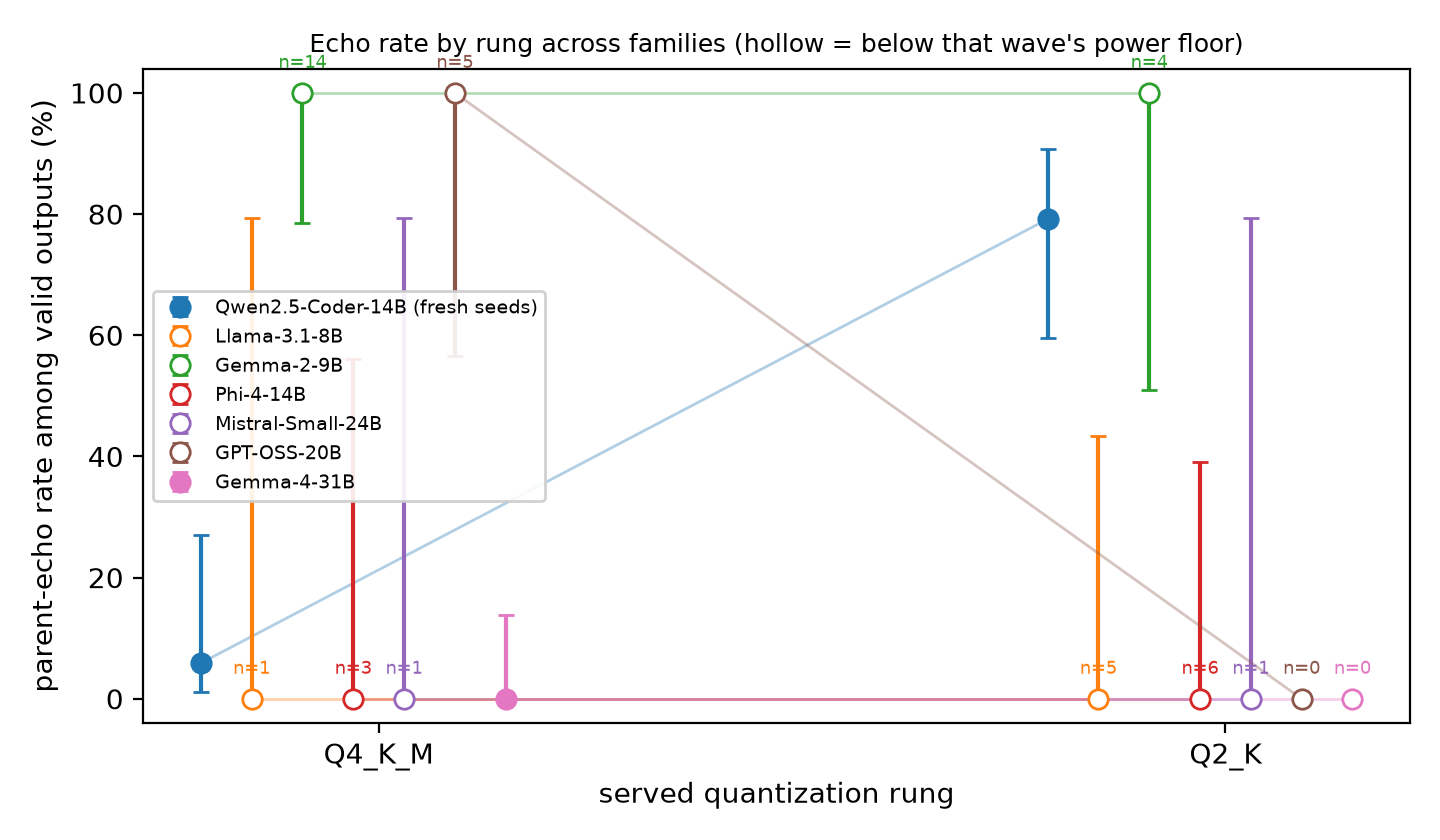
\includegraphics[width=\linewidth]{fig4_family_echo}
\caption{Coordinate-verified parent-echo among valid outputs, by rung, across every family ladder in the programme, replayed from the raw ledgers (each family judged against its own registration's power floor). Qwen's fresh-seed wave carries the registered contrast (1/17 at Q4\_K\_M against 19/24 at Q2\_K); gemma-2 echoes every output it validates at both rungs (14/14, 4/4); gpt-oss echoes all five of its Q4\_K\_M validities; gemma-4 echoes none of its 24 and validates nothing at Q2\_K; Llama, Phi-4 and Mistral sit below their competence floors. Across the families that clear their floors the pattern is consistent with family-shaped echo and family-shaped 2-bit failure channels; the below-floor bars cannot speak to either, and no bar here is a registered verdict.}
\label{fig:family-echo}
\end{figure}

Finally, \S3's data comes from a locally-served open-weights ladder at $N = 26$, not from the alias-addressed runtime and not at \S4's cells ($N = 13, 21, 31$). The mechanism gap --- that served quantization matters for this task --- is supported by \S3's measurement rather than measured inside the runtime, which is exactly the measurement \S5 says cannot be made. The instance gap --- that a cliff observed at $N = 26$ transfers to $N = 13/21/31$ --- is supported by the companion paper's finding that the same constructible template family governs proposals across $N$, but is an inference, not a replication. A reader should treat \S3 as establishing that the failure mode \emph{exists and is invisible to pass/fail metrics}, and treat its quantitative rungs as belonging to the sweep, not to \S4.

\section*{Use of AI systems}

This paper studies language-model behaviour and was written with language-model assistance. Claude models wrote the collection, scoring and analysis scripts and drafted the manuscript prose; the human author directed the programme, approved each preregistration before sampling, made the final inclusion, stopping and submission decisions, and is solely responsible for the content. Internal adversarial checks by language models of other families preceded submission; they are quality assurance, not review, and carry no external authority. The claim a reader can check is the ordering, not the authorship --- each preregistration commit is a git ancestor of the sampling it governs --- and because the authoring models share a family with the runtime under study in \S4, the released scripts, raw ledgers and frozen outputs, rather than the authorship, are what the claims rest on.
